\ifx\pdfminorversion\undefined\else\pdfminorversion=4\fi
\documentclass[aspectratio=169,t,xcolor=dvipsnames]{beamer}
%\documentclass[aspectratio=169,t,handout]{beamer}

% English version FAU Logo
\usepackage[english]{babel}
% German version FAU Logo
%\usepackage[ngerman]{babel}

\usepackage[utf8]{inputenc}
\usepackage[T1]{fontenc}
\usepackage{amsmath,amssymb}
\usepackage{graphicx}
\usepackage{listings}
\usepackage{url}
\usepackage{enumitem}
\usepackage{hyperref}
\usepackage{fontawesome}
\usepackage{graphicx}
\usepackage{booktabs}
\usepackage{calc}
\usepackage{ifthen}
\usepackage{xcolor}
\usepackage{tabularx}
\usepackage{makecell}
\usepackage{tikz}
\usepackage{tikz}
\usepackage{tikz-cd}
\usepackage{verbatim}
\usepackage{pgfplots,pgfplotstable,pgf-pie}
\usepackage{filecontents}
\newcommand{\plots}{0.611201}
\newcommand{\plotm}{2.19882}
\pgfplotsset{height=4cm,width=8cm,compat=1.16}
\pgfmathdeclarefunction{gauss}{2}{%
  \pgfmathparse{1/(#2*sqrt(2*pi))*exp(-((x-#1)^2)/(2*#2^2))}%
}

\tikzset{
    vertex/.style = {
        circle,
        fill            = black,
        outer sep = 2pt,
        inner sep = 1pt,
    }
}

\tikzset{
    mynode/.style={
        draw,
        thick,
        anchor=south west,
        minimum width=2cm,
        minimum height=1.3cm,
        align=center,
        inner sep=0.2cm,
        outer sep=0,
        rectangle split,
        rectangle split parts=2,
        rectangle split draw splits=false},
    reverseclip/.style={
        insert path={(current page.north east) --
            (current page.south east) --
            (current page.south west) --
            (current page.north west) --
            (current page.north east)}
    }
}

\tikzset{basic/.style={
        draw,
        rectangle split,
        rectangle split parts=2,
        rectangle split part fill={blue!20,white},
        minimum width=2.5cm,
        text width=2cm,
        align=left,
        font=\itshape
    },
    Diamond/.style={ diamond,
                      draw,
                      shape aspect=2,
                      inner sep = 2pt,
                      text centered,
                      fill=blue!10!white,
                      font=\itshape
                    }}


\tikzset{level 1/.append style={sibling angle=50,level distance = 165mm}}
\tikzset{level 2/.append style={sibling angle=20,level distance = 45mm}}
\tikzset{every node/.append style={scale=1}}

\usetikzlibrary{arrows,decorations.pathmorphing,backgrounds,fit,positioning,shapes.symbols,chains,intersections,snakes,positioning,matrix,mindmap,shapes.multipart,shapes,calc,shapes.geometric}

% read in data file


\newcommand{\MaxNumberX}{3}
\newcommand{\MaxNumberY}{5}
\newcommand{\tikzmark}[1]{\tikz[remember picture] \node[coordinate] (#1) {#1};}

\pgfplotstableread{data/iris.dat}\iris
\pgfplotstablegetrowsof{\iris}
\pgfplotsset{compat=1.14}
\pgfmathsetmacro\NumRows{\pgfplotsretval-1}
\definecolor{airforceblue}{rgb}{0.36, 0.54, 0.66}

\usepgfplotslibrary{groupplots}
% Options:
%  - inst:      Institute
%                 med:      MedFak FAU theme
%                 nat:      NatFak FAU theme
%                 phil:     PhilFak FAU theme
%                 rw:       RWFak FAU theme
%                 rw-jura:  RWFak FB Jura FAU theme
%                 rw-wiso:  RWFak FB WISO FAU theme
%                 tf:       TechFak FAU theme
%  - image:     Cover image on title page
%  - plain:     Plain title page
%  - longtitle: Title page layout for long title
\usetheme[%
  image,%
  longtitle,%
  tf
]{fau}

% Enable semi-transparent animation preview
\setbeamercovered{transparent}


\lstset{%
  language=Python,
  tabsize=2,
  basicstyle=\tt,
  keywordstyle=\color{blue},
  commentstyle=\color{green!50!black},
  stringstyle=\color{red},
  numbers=left,
  numbersep=0.5em,
  xleftmargin=1em,
  numberstyle=\tt
}


% Title, authors, and date
\title[KDD]{Chapter VII: Cluster analysis}
\subtitle{Knowledge Discovery in Databases}
\author[L.~Melodia]{Luciano Melodia M.A.}
% English version
\institute[Department]{Evolutionary Data Management, Friedrich-Alexander University Erlangen-Nürnberg}
% German version
%\institute[Lehrstuhl]{Lehrstuhl, Friedrich-Alexander-Universit\"at Erlangen-N\"urnberg}
\date{Summer semester 2021}
% Set additional logo (overwrites FAU seal)
%\logo{\includegraphics[width=.15\textwidth]{themefau/art/xxx/xxx.pdf}}
\begin{document}
  % Title
  \maketitle

  {
    \setbeamertemplate{footline}{}
    \begin{frame}{Chapter VII: Cluster analysis}
        \begin{itemize}
            \item \textbf{Cluster analysis: basic concepts.}
            \item Partitioning methods.
            \item Hierarchical methods.
            \item Density-based methods.
            \item Grid-based methods.
            \item Evaluation of clustering.
            \item Summary.
        \end{itemize}
    \end{frame}
  }

  {
    \setbeamertemplate{footline}{}
    \begin{frame}{What is cluster analysis?}
        \begin{itemize}
          \item \textbf{{\color{airforceblue}Cluster}: A collection of data objects within a larger set that are.}
          \begin{itemize}
            \item {\color{airforceblue}Similar (or related)} to one another within the same group and,
            \item dissimilar (or unrelated) to the objects outside the group.
          \end{itemize}
          \item \textbf{{\color{airforceblue}Cluster analysis} (or clustering, data segmentation, $\ldots$).}
          \begin{itemize}
            \item {\color{airforceblue}Define similarities} among data based on the characteristics found in the data (input from user!).
            \item Group similar data objects into clusters.
          \end{itemize}
          \item \textbf{Unsupervised learning:}
          \begin{itemize}
            \item No predefined classes.
            \item I.e., learning by observation (vs. learning by examples: supervised).
          \end{itemize}
          \item \textbf{Typical applications:}
          \begin{itemize}
            \item As a stand-alone tool to get insight into data distribution.
            \item As a preprocessing step for other algorithms.
          \end{itemize}
        \end{itemize}
    \end{frame}
  }

  {
    \setbeamertemplate{footline}{}
    \begin{frame}{Clustering for data understanding and applications}
        \begin{itemize}
          \item \textbf{Biology:}
          \begin{itemize}
            \item Taxonomy of living things: kingdom, phylum, class, order, family, genus, and species.
          \end{itemize}
          \item \textbf{Information retrieval:}
          \begin{itemize}
            \item Document clustering.
          \end{itemize}
          \item \textbf{Land use:}
          \begin{itemize}
            \item Identification of areas of similar land use in an earth-observation database.
          \end{itemize}
          \item \textbf{Marketing:}
          \begin{itemize}
            \item Help marketers discover distinct groups in their customer bases, and then use this knowledge to develop targeted marketing programs.
          \end{itemize}
          \item \textbf{City planning:}
          \begin{itemize}
            \item Identifying groups of houses according to their house type, value, and geographical location.
          \end{itemize}
          \item \textbf{Earthquake studies:}
          \begin{itemize}
            \item Observed earthquake epicenters should be clustered along continent faults.
          \end{itemize}
          \item \textbf{Climate:}
          \begin{itemize}
            \item Understanding earth climate, find patterns of atmosphere and ocean.
          \end{itemize}
        \end{itemize}
    \end{frame}
  }

  {
    \setbeamertemplate{footline}{}
    \begin{frame}{Quality: what is good clustering?}
        \begin{itemize}
          \item \textbf{A good clustering method will produce high-quality clusters.}
          \begin{itemize}
            \item \textbf{\color{airforceblue}High intra-class similarity:}
            \begin{itemize}
              \item Cohesive within clusters.
            \end{itemize}
            \item \textbf{\color{airforceblue}Low inter-class similarity:}
            \begin{itemize}
              \item Distinctive between clusters.
            \end{itemize}
          \end{itemize}
          \item \textbf{The {\color{airforceblue}quality} of a clustering method depends on:}
          \begin{itemize}
            \item the \textbf{\color{airforceblue}similarity measure} used by the method,
            \item its implementation, and
            \item its ability to discover some or all of the hidden patterns.
          \end{itemize}
        \end{itemize}
    \end{frame}
  }

  {
    \setbeamertemplate{footline}{}
    \begin{frame}{Measure the quality of clustering}
        \begin{itemize}
          \item \textbf{Dissimilarity/similarity metric:}
          \begin{itemize}
            \item Similarity is expressed in terms of a distance function, typically a metric: $d(x,y)$.
            \item The definitions of distance functions are usually rather different for interval-scaled, Boolean, categorical, ordinal, ratio, and vector variables (see chapter 2).
            \item \textbf{\color{airforceblue}Weights} should be associated with different variables \\
                  based on applications and data semantics.
          \end{itemize}
          \item \textbf{Quality of clustering:}
          \begin{itemize}
            \item There is usually a separate \textbf{\color{airforceblue}"quality" function} that measures the "goodness" of a cluster.
            \item It is hard to define "similar enough" or "good enough."
            \item The answer is typically highly subjective.
          \end{itemize}
        \end{itemize}
    \end{frame}
  }

  {
    \setbeamertemplate{footline}{}
    \begin{frame}{Considerations for cluster analysis}
        \begin{itemize}
          \item \textbf{Partitioning criteria:}
          \begin{itemize}
            \item Single level vs. hierarchical partitioning.
            \item Often, multi-level hierarchical partitioning is desirable.
          \end{itemize}
          \item \textbf{Separation of clusters:}
          \begin{itemize}
            \item Exclusive (e.g., one customer belongs to only one region) vs.
            \item Non-exclusive (e.g., one document may belong to more than one class).
          \end{itemize}
          \item \textbf{Similarity measure:}
          \begin{itemize}
            \item Distance-based (e.g., Euclidian, road network, vector) vs.
            \item Connectivity-based (e.g., density or contiguity).
          \end{itemize}
          \item \textbf{Clustering space:}
          \begin{itemize}
            \item Full space (often when low-dimensional) vs.
            \item Subspaces (often in high-dimensional clustering).
          \end{itemize}
        \end{itemize}
    \end{frame}
  }

  {
    \setbeamertemplate{footline}{}
    \begin{frame}{Requirements and challenges}
        \begin{itemize}
          \item \textbf{Scalability:}
          \begin{itemize}
            \item Clustering all the data instead of only on samples.
          \end{itemize}
          \item \textbf{Ability to deal with different types of attributes:}
          \begin{itemize}
            \item Numerical, binary, categorical, ordinal, linked, and mixture of these.
          \end{itemize}
          \item \textbf{Constraint-based clustering:}
          \begin{itemize}
            \item User may give inputs on constraints.
            \item Use domain knowledge to determine input parameters.
          \end{itemize}
          \item \textbf{Interpretability and usability.}
          \item \textbf{Others:}
          \begin{itemize}
            \item Discovery of clusters with arbitrary shape.
            \item Ability to deal with noisy data.
            \item Incremental clustering and insensitivity to input order.
            \item High dimensionality.
          \end{itemize}
        \end{itemize}
    \end{frame}
  }

  {
    \setbeamertemplate{footline}{}
    \begin{frame}{Major clustering approaches}
        \begin{itemize}
          \item \textbf{Partitioning approach:}
          \begin{itemize}
            \item Construct various partitions and then evaluate them by some criterion.
            \item E.g., minimizing the sum of square errors.
            \item Typical methods: k-means, k-medoids, CLARA, CLARANS.
          \end{itemize}
          \item \textbf{Hierarchical approach:}
          \begin{itemize}
            \item Create a hierarchical decomposition of the set of data (or objects) using some criterion.
            \item Typical methods: AGNES, DIANA, BIRCH, CHAMELEON.
          \end{itemize}
          \item \textbf{Density-based approach:}
          \begin{itemize}
            \item Based on connectivity and density functions.
            \item Typical methods: DBSCAN, OPTICS, DENCLUE.
          \end{itemize}
          \item \textbf{Grid-based approach:}
          \begin{itemize}
            \item Based on a multiple-level granularity structure.
            \item Typical methods: STING, WaveCluster, CLIQUE.
          \end{itemize}
        \end{itemize}
    \end{frame}
  }

  {
    \setbeamertemplate{footline}{}
    \begin{frame}{Major clustering approaches (II)}
        \begin{itemize}
          \item \textbf{Model-based approach:}
          \begin{itemize}
            \item A model is hypothesized for each of the clusters and tries to find the best fit of that model to each other.
            \item Typical methods: EM, SOM, COBWEB.
          \end{itemize}
          \item \textbf{Frequent-pattern-based approach:}
          \begin{itemize}
            \item Based on the analysis of frequent patterns.
            \item Typical methods: p-Cluster.
          \end{itemize}
          \item \textbf{User-guided or constraint-based approach:}
          \begin{itemize}
            \item Clustering by considering user-specified or application-specific constraints.
            \item Typical methods: COD (obstacles), constrained clustering.
          \end{itemize}
          \item \textbf{Link-based clustering:}
          \begin{itemize}
            \item Objects are often linked together in various ways.
            \item Massive links can be used to cluster objects: SimRank, LinkClus.
          \end{itemize}
        \end{itemize}
    \end{frame}
  }

  {
    \setbeamertemplate{footline}{}
    \begin{frame}{Chapter VII: Cluster analysis}
        \begin{itemize}
            \item Cluster analysis: basic concepts.
            \item \textbf{Partitioning methods.}
            \item Hierarchical methods.
            \item Density-based methods.
            \item Grid-based methods.
            \item Evaluation of clustering.
            \item Summary.
        \end{itemize}
    \end{frame}
  }

  {
    \setbeamertemplate{footline}{}
    \begin{frame}{Partitioning algorithms: basic concept}
        \begin{itemize}
          \item \textbf{Partitioning method:}
          \begin{itemize}
            \item Partition a database $D$ of $n$ objects $o_j, j \in \{1, \ldots, n\}$ into a set of $k$-clusters $C_i$, $1 \leq i \leq k$ such that the sum of squared distances to $c_i$ is minimized \\ (where $c_i$ is the \textbf{\color{airforceblue}centroid} or \textbf{\color{airforceblue}medoid} of cluster $C_i$):
            \begin{align}
              \min \sum_{i=1}^{k} \sum_{o \in C_i} d(o,c_i)^2.
            \end{align}
          \end{itemize}
          \item \textbf{Given $k$, find a partition of $k$ clusters that optimizes the chosen partitioning criterion.}
          \begin{itemize}
            \item Globally optimal: exhaustively enumerate all partitions.
            \item Heuristic methods: k-means and k-medoids algorithms.
            \item \textbf{\color{airforceblue}k-means} (MacQueen'67, Lloyd'57/'82):
            \begin{itemize}
              \item Each cluster is represented by the center of the cluster.
            \end{itemize}
            \item \textbf{\color{airforceblue}k-medoids} or PAM (Partition around medoids) (Kaufman \& Rousseeuw'87):
            \begin{itemize}
              \item Each cluster is represented by one of the objects in the cluster.
            \end{itemize}
          \end{itemize}
        \end{itemize}
    \end{frame}
  }

  {
    \setbeamertemplate{footline}{}
    \begin{frame}{The $k$-means clustering method}
        \begin{itemize}
          \item \textbf{Given $k$, the $k$-means algorithm is implemented in four steps:}
          \begin{itemize}
            \item[1.] Partition the database into $k$ non-empty subsets.
            \begin{itemize}
              \item E.g. the first $\frac{n}{k}$ objects, then the next $\frac{n}{k}$ objects, $\ldots$
            \end{itemize}
            \item[2.] Compute the centroids of the \textbf{clusters} of the current partitioning.
            \begin{itemize}
              \item The centroid is the center, i.e. mean point, of the cluster.
              \item For each attribute (or dimension), calculate the average value.
            \end{itemize}
            \item[3.] Assign each object to the cluster with the nearest centroid.
            \begin{itemize}
              \item That is, for each object calculate distance to each of the $k$\\
              centroids and pick the one with the smallest distance.
            \end{itemize}
          \item[4.] If any object has changed its cluster, go back to step 2. Otherwise stop.
          \end{itemize}
          \item \textbf{Variant:}
          \begin{itemize}
            \item Start with arbitrarily chosen $k$ objects as initial centroids in step $1$.
            \item Continue with step $3$.
          \end{itemize}
        \end{itemize}
    \end{frame}
  }

  {
    \setbeamertemplate{footline}{}
    \begin{frame}{An example of $k$-means clustering}
      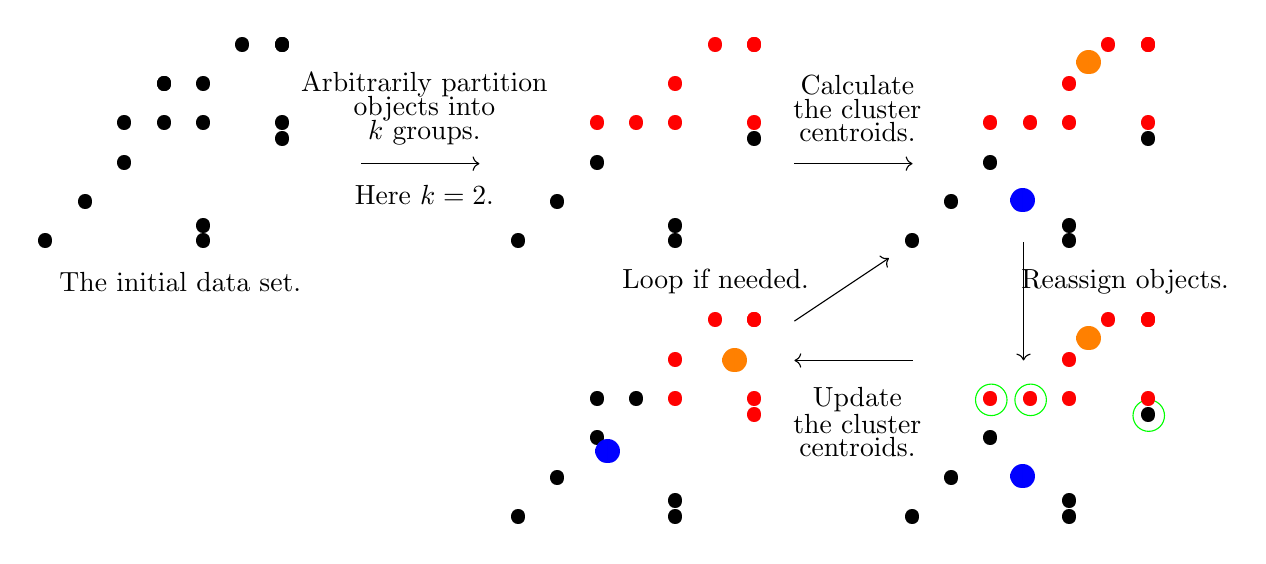
\begin{tikzpicture}
        \node [black] at (3,2.5) {\Large\textbullet};
        \node [black] at (4,3.5) {\Large\textbullet};
        \node [black] at (2,2.5) {\Large\textbullet};
        \node [black] at (2.5,3) {\Large\textbullet};
        \node [black] at (3,1) {\Large\textbullet};
        \node [black] at (3,1.2) {\Large\textbullet};
        \node [black] at (1,1) {\Large\textbullet};
        \node [black] at (1.5,1.5) {\Large\textbullet};
        \node [black] at (2,2) {\Large\textbullet};
        \node [black] at (2.5,2.5) {\Large\textbullet};
        \node [black] at (3,3) {\Large\textbullet};
        \node [black] at (3.5,3.5) {\Large\textbullet};
        \node [black] at (4,3.5) {\Large\textbullet};
        \node [black] at (4,2.3) {\Large\textbullet};
        \node [black] at (4,2.5) {\Large\textbullet};
        \node [black] at (2.5,3) {\Large\textbullet};
        \node [black] at (2.7,0.5) {The initial data set.};

        \node [black] at (7,1) {\Large\textbullet};
        \node [black] at (7.5,1.5) {\Large\textbullet};
        \node [black] at (8,2) {\Large\textbullet};
        \node [red] at (8,2.5) {\Large\textbullet};
        \node [red] at (8.5,2.5) {\Large\textbullet};
        \node [black] at (9,1) {\Large\textbullet};
        \node [black] at (9,1.2) {\Large\textbullet};
        \node [red] at (9,2.5) {\Large\textbullet};
        \node [red] at (9,3) {\Large\textbullet};
        \node [red] at (9.5,3.5) {\Large\textbullet};
        \node [red] at (10,3.5) {\Large\textbullet};
        \node [red] at (10,3.5) {\Large\textbullet};
        \node [black] at (10,2.3) {\Large\textbullet};
        \node [red] at (10,2.5) {\Large\textbullet};

        \node [black] at (12,1) {\Large\textbullet};
        \node [black] at (12.5,1.5) {\Large\textbullet};
        \node [black] at (13,2) {\Large\textbullet};
        \node [red] at (13,2.5) {\Large\textbullet};
        \node [red] at (13.5,2.5) {\Large\textbullet};
        \node [black] at (14,1) {\Large\textbullet};
        \node [black] at (14,1.2) {\Large\textbullet};
        \node [red] at (14,2.5) {\Large\textbullet};
        \node [red] at (14,3) {\Large\textbullet};
        \node [red] at (14.5,3.5) {\Large\textbullet};
        \node [red] at (15,3.5) {\Large\textbullet};
        \node [red] at (15,3.5) {\Large\textbullet};
        \node [black] at (15,2.3) {\Large\textbullet};
        \node [red] at (15,2.5) {\Large\textbullet};
        \node [orange] at (14.25,3.25) {\Huge\textbullet};
        \node [blue] at (13.41,1.5) {\Huge\textbullet};

        \node [black] at (12,-2.5) {\Large\textbullet};
        \node [black] at (12.5,-2) {\Large\textbullet};
        \node [black] at (13,-1.5) {\Large\textbullet};
        \node [red] at (13,-1) {\Large\textbullet};
        \node [red] at (13.5,-1) {\Large\textbullet};
        \draw[green] (13,-1) circle (0.2cm);
        \draw[green] (13.5,-1) circle (0.2cm);
        \node [black] at (14,-2.5) {\Large\textbullet};
        \node [black] at (14,-2.3) {\Large\textbullet};
        \node [red] at (14,-1) {\Large\textbullet};
        \node [red] at (14,-0.5) {\Large\textbullet};
        \node [red] at (14.5,0) {\Large\textbullet};
        \node [red] at (15,0) {\Large\textbullet};
        \node [red] at (15,0) {\Large\textbullet};
        \node [black] at (15,-1.2) {\Large\textbullet};
        \draw[green] (15,-1.2) circle (0.2cm);
        \node [red] at (15,-1) {\Large\textbullet};
        \node [orange] at (14.25,-0.25) {\Huge\textbullet};
        \node [blue] at (13.41,-2) {\Huge\textbullet};

        \node [black] at (7,-2.5) {\Large\textbullet};
        \node [black] at (7.5,-2) {\Large\textbullet};
        \node [black] at (8,-1.5) {\Large\textbullet};
        \node [black] at (8,-1) {\Large\textbullet};
        \node [black] at (8.5,-1) {\Large\textbullet};
        \node [black] at (9,-2.5) {\Large\textbullet};
        \node [black] at (9,-2.3) {\Large\textbullet};
        \node [red] at (9,-1) {\Large\textbullet};
        \node [red] at (9,-0.5) {\Large\textbullet};
        \node [red] at (9.5,0) {\Large\textbullet};
        \node [red] at (10,0) {\Large\textbullet};
        \node [red] at (10,0) {\Large\textbullet};
        \node [red] at (10,-1.2) {\Large\textbullet};
        \node [red] at (10,-1) {\Large\textbullet};
        \node [orange] at (9.75,-0.53) {\Huge\textbullet};
        \node [blue] at (8.14,-1.68) {\Huge\textbullet};

        \draw [->] (13.41,1) -- (13.41,-0.5);
        \node [black] at (14.7,0.5) {Reassign objects.};

        \draw [->] (5,2) -- (6.5,2);
        \node [black] at (5.8,3) {Arbitrarily partition};
        \node [black] at (5.8,2.7) {objects into};
        \node [black] at (5.8,2.4) {$k$ groups.};
        \node [black] at (5.8,1.6) {Here $k = 2$.};

        \draw [->] (10.5,2) -- (12,2);
        \node [black] at (11.3,3) {Calculate};
        \node [black] at (11.3,2.7) {the cluster};
        \node [black] at (11.3,2.4) {centroids.};

        \draw [->]  (12,-0.5) -- (10.5,-0.5);
        \draw [->]  (10.5,0)--(11.7,0.8);
        \node [black] at (9.5,0.5) {Loop if needed.};
        \node [black] at (11.3,-1) {Update};
        \node [black] at (11.3,-1.3) {the cluster};
        \node [black] at (11.3,-1.6) {centroids.};
      \end{tikzpicture}
    \end{frame}
  }

  {
    \setbeamertemplate{footline}{}
    \begin{frame}{Comments on the $k$-means method}
      \begin{itemize}
        \item \textbf{Strength:}
        \begin{itemize}
          \item Efficient: $\mathcal{O}(tkn)$, where $n$ is $\#$ objects, $k$ is $\#$ of clusters, and $t$ is the $\#$ of iterations. Normally, $k$, $t \ll n$.
          \item Comparing: PAM: $\mathcal{O}(k(n-k)^2)$, CLARA: $\mathcal{O}(ks^2 + k(n-k))$.
          \item Comment: Often terminates at a local optimum.
        \end{itemize}
        \item \textbf{Weakness:}
        \begin{itemize}
          \item Applicable only to objects in a continuous n-dimensional space.
          \begin{itemize}
            \item Using the $k$-modes method for categorical data.
            \item In comparison, $k$-medoids can be applied to a wide range of data.
          \end{itemize}
          \item Need to specify $k$, the number of clusters, in advance.
          \begin{itemize}
            \item There are ways to automatically determine the best $k$ (see Hastie et al., 2009).
          \end{itemize}
          \item Sensitive to noisy data and outliers.
          \item Not suitable to discover clusters with non-convex shapes.
        \end{itemize}
      \end{itemize}
    \end{frame}
  }

  {
    \setbeamertemplate{footline}{}
    \begin{frame}{Variations of the $k$-means method}
      \begin{itemize}
        \item \textbf{Most of the variants of the $k$-means differ in:}
        \begin{itemize}
          \item Selection of the initial $k$ subsets (or centroids).
          \item Dissimilarity calculations.
          \item Strategies to calculate cluster centroids.
        \end{itemize}
        \item \textbf{Handling categorical data: $k$-modes:}
        \begin{itemize}
          \item Replacing centroids with modes.
          \begin{itemize}
            \item See Chapter 2: mode = value that occurs most frequently in the data.
          \end{itemize}
          \item Using new dissimilarity measures to deal with categorical objects.
          \item Using a frequency-based method to update modes of clusters.
          \item A mixture of categorical and numerical data: k-prototype method.
        \end{itemize}
      \end{itemize}
    \end{frame}
  }

  {
    \setbeamertemplate{footline}{}
    \begin{frame}{What is the problem of the $k$-means method?}
      \begin{itemize}
        \item \textbf{The $k$-means algorithm is {\color{airforceblue}sensitive to outliers}!}
        \begin{itemize}
          \item Since an object with an extremely large value may substantially \\
          distort the distribution of the data.
        \end{itemize}
        \item \textbf{$k$-medoids:}
        \begin{itemize}
          \item Instead of taking the mean value of the objects in a cluster as a reference point,\\
          medoids can be used, which is the most centrally located object in a cluster.
        \end{itemize}
      \end{itemize}
      \centering
      \newcommand*{\xMin}{0}%
      \newcommand*{\xMax}{10}%
      \newcommand*{\yMin}{0}%
      \newcommand*{\yMax}{10}%
      \begin{tikzpicture}[scale=0.3]
          \foreach \i in {\xMin,...,\xMax} {
              \draw [very thin,gray] (\i,\yMin) -- (\i,\yMax)  node [below] at (\i,\yMin) {\tiny$\i$};
          }
          \foreach \i in {\yMin,...,\yMax} {
              \draw [very thin,gray] (\xMin,\i) -- (\xMax,\i) node [left] at (\xMin,\i) {\tiny$\i$};
          }
          \node[color=orange] at (4,3) {\Huge\textbullet};
          \node[color=orange] at (3,6) {\Huge\textbullet};
          \node[color=orange] at (3,8) {\Huge\textbullet};
          \node[color=orange] at (4,7) {\Huge\textbullet};
          \node[color=orange] at (4,5) {\Huge\textbullet};
          \node[color=orange] at (5,5) {\Huge\textbullet};
          \node[color=blue] at (5,1) {\Huge\textbullet};
          \node[color=blue] at (7,3) {\Huge\textbullet};
          \node[color=blue] at (7,4) {\Huge\textbullet};
          \node[color=blue] at (8,5) {\Huge\textbullet};
          \draw[->] (12,5)--(17,5);
      \end{tikzpicture}
      \begin{tikzpicture}[scale=0.3]
          \foreach \i in {\xMin,...,\xMax} {
              \draw [very thin,gray] (\i,\yMin) -- (\i,\yMax)  node [below] at (\i,\yMin) {\tiny$\i$};
          }
          \foreach \i in {\yMin,...,\yMax} {
              \draw [very thin,gray] (\xMin,\i) -- (\xMax,\i) node [left] at (\xMin,\i) {\tiny$\i$};
          }
          \node[color=orange] at (4,3) {\Large\textbullet};
          \node[color=red] at (3,6) {\Huge\textbullet};
          \node[color=orange] at (3,8) {\Large\textbullet};
          \node[color=orange] at (4,7) {\Large\textbullet};
          \node[color=orange] at (4,5) {\Large\textbullet};
          \node[color=orange] at (5,5) {\Large\textbullet};
          \node[color=blue] at (5,1) {\Large\textbullet};
          \node[color=blue] at (7,3) {\Huge\textbullet};
          \node[color=blue] at (7,4) {\Large\textbullet};
          \node[color=blue] at (8,5) {\Large\textbullet};
      \end{tikzpicture}
    \end{frame}
  }

  {
    \setbeamertemplate{footline}{}
    \begin{frame}{The $k$-medoids clustering method}
      \begin{itemize}
        \item \textbf{$k$-medoids clustering:}
        \begin{itemize}
          \item Find representative objects (medoids) in clusters.
          \item \textbf{PAM} (Partitioning Around Medoids, Kaufmann \& Rousseeuw, 1987):
            \begin{itemize}
              \item Starts from an initial set of $k$ medoids and iteratively replaces one of the medoids \\
              by one of the non-medoids, if it improves the total distance of the resulting clustering.
              \item PAM works effectively for small data sets, but does not scale well for large\\
              data sets (due to the computational complexity).
            \end{itemize}
            \end{itemize}
        \item \textbf{Efficiency improvement on PAM:}
        \begin{itemize}
          \item CLARA (Kaufmann \& Rousseeuw, 1990): PAM on samples.
          \item CLARANS (Ng \& Han, 1994): Randomized re-sampling.
        \end{itemize}
      \end{itemize}
    \end{frame}
  }

  {
    \setbeamertemplate{footline}{}
    \begin{frame}{PAM: A typical $k$-medoids algorithm}
      \newcommand*{\xMin}{0}%
      \newcommand*{\xMax}{10}%
      \newcommand*{\yMin}{0}%
      \newcommand*{\yMax}{10}%
      \centering
      \begin{tikzpicture}[scale=0.23]
          \foreach \i in {\xMin,...,\xMax} {
              \draw [very thin,gray] (\i,\yMin) -- (\i,\yMax)  node [below] at (\i,\yMin) {\tiny$\i$};
          }
          \foreach \i in {\yMin,...,\yMax} {
              \draw [very thin,gray] (\xMin,\i) -- (\xMax,\i) node [left] at (\xMin,\i) {\tiny$\i$};
          }
          \node[color=orange] at (2,6) {\Large\textbullet};
          \node[color=orange] at (3,4) {\Large\textbullet};
          \node[color=orange] at (3,8) {\Large\textbullet};
          \node[color=orange] at (4,7) {\Large\textbullet};
          \node[color=orange] at (6,2) {\Large\textbullet};
          \node[color=orange] at (6,3) {\Large\textbullet};
          \node[color=orange] at (7,3) {\Large\textbullet};
          \node[color=orange] at (7,4) {\Large\textbullet};
          \node[color=orange] at (7,6) {\Large\textbullet};
          \node[color=orange] at (8,5) {\Large\textbullet};
          \draw[->] (12,3)--(17,3);
          \node at (14,8) {\scriptsize Arbitrarily};
          \node at (14,7) {\scriptsize choose $k$};
          \node at (14,6) {\scriptsize object as};
          \node at (14,5) {\scriptsize initial};
          \node at (14,4) {\scriptsize medoids};
          \node at (14,2) {\scriptsize for $k=2$};
      \end{tikzpicture}
      \begin{tikzpicture}[scale=0.23]
          \foreach \i in {\xMin,...,\xMax} {
              \draw [very thin,gray] (\i,\yMin) -- (\i,\yMax)  node [below] at (\i,\yMin) {\tiny$\i$};
          }
          \foreach \i in {\yMin,...,\yMax} {
              \draw [very thin,gray] (\xMin,\i) -- (\xMax,\i) node [left] at (\xMin,\i) {\tiny$\i$};
          }
          \node[color=orange] at (2,6) {\Large\textbullet};
          \node[color=orange] at (3,4) {\Large\textbullet};
          \node[color=blue] at (3,8) {\Large\textbullet};
          \node[color=orange] at (4,7) {\Large\textbullet};
          \node[color=orange] at (6,2) {\Large\textbullet};
          \node[color=blue] at (6,3) {\Large\textbullet};
          \node[color=orange] at (7,3) {\Large\textbullet};
          \node[color=orange] at (7,4) {\Large\textbullet};
          \node[color=orange] at (7,6) {\Large\textbullet};
          \node[color=orange] at (8,5) {\Large\textbullet};
          \draw[->] (12,3)--(17,3);
          \node at (14,8) {\scriptsize Assign};
          \node at (14,7) {\scriptsize each};
          \node at (14,6) {\scriptsize remaining};
          \node at (14,5) {\scriptsize object to};
          \node at (14,4) {\scriptsize nearest medoid};
      \end{tikzpicture}
      \begin{tikzpicture}[scale=0.23]
          \foreach \i in {\xMin,...,\xMax} {
              \draw [very thin,gray] (\i,\yMin) -- (\i,\yMax)  node [below] at (\i,\yMin) {\tiny$\i$};
          }
          \foreach \i in {\yMin,...,\yMax} {
              \draw [very thin,gray] (\xMin,\i) -- (\xMax,\i) node [left] at (\xMin,\i) {\tiny$\i$};
          }
          \node[color=orange] at (2,6) {\Large\textbullet};
          \node[color=orange] at (3,4) {\Large\textbullet};
          \node[color=blue] at (3,8) {\Large\textbullet};
          \node[color=orange] at (4,7) {\Large\textbullet};
          \node[color=orange] at (6,2) {\Large\textbullet};
          \node[color=blue] at (6,3) {\Large\textbullet};
          \node[color=orange] at (7,3) {\Large\textbullet};
          \node[color=orange] at (7,4) {\Large\textbullet};
          \node[color=orange] at (7,6) {\Large\textbullet};
          \node[color=orange] at (8,5) {\Large\textbullet};
          \draw[dashed] (3,6) ellipse (2cm and 3cm);
          \draw[dashed] (7,4) ellipse (2cm and 3cm);
          \draw[->] (12,3) to [out=30,in=30] (12,-1);
          \node at (7,11) {\scriptsize Total cost = 20};
          \node at (15,8) {\scriptsize Randomly};
          \node at (15,7) {\scriptsize select};
          \node at (15,6) {\scriptsize nonmedoid};
          \node at (15,5) {\scriptsize object $o_\text{random}$};
      \end{tikzpicture}\\
      \hspace{1.2cm}
      \begin{tikzpicture}[scale=0.23]
          \foreach \i in {\xMin,...,\xMax} {
              \draw [very thin,gray] (\i,\yMin) -- (\i,\yMax)  node [below] at (\i,\yMin) {\tiny$\i$};
          }
          \foreach \i in {\yMin,...,\yMax} {
              \draw [very thin,gray] (\xMin,\i) -- (\xMax,\i) node [left] at (\xMin,\i) {\tiny$\i$};
          }
          \node[color=orange] at (2,6) {\Large\textbullet};
          \node[color=orange] at (3,4) {\Large\textbullet};
          \node[color=blue] at (3,8) {\Large\textbullet};
          \node[color=orange] at (4,7) {\Large\textbullet};
          \node[color=red] at (6,2) {\Large\textbullet};
          \node[color=blue] at (6,3) {\Large\textbullet};
          \node[color=orange] at (7,3) {\Large\textbullet};
          \node[color=green] at (7,4) {\Large\textbullet};
          \node[color=orange] at (7,6) {\Large\textbullet};
          \node[color=orange] at (8,5) {\Large\textbullet};
          \draw[->] (17,5)--(12,5);
          \draw[->] (12,6)--(17,10);
          \node at (15,4) {\scriptsize Compute};
          \node at (15,3) {\scriptsize total cost of};
          \node at (15,2) {\scriptsize swapping};
          \node at (-5,4) {\scriptsize Swapping $o$};
          \node at (-5,3) {\scriptsize and $o_\text{random}$};
          \node at (-5,2) {\scriptsize if quality is};
          \node at (-5,1) {\scriptsize improved};
          \node at (3.4,11) {\scriptsize Total cost = 26};
      \end{tikzpicture}
      \begin{tikzpicture}[scale=0.23]
          \foreach \i in {\xMin,...,\xMax} {
              \draw [very thin,gray] (\i,\yMin) -- (\i,\yMax)  node [below] at (\i,\yMin) {\tiny$\i$};
          }
          \foreach \i in {\yMin,...,\yMax} {
              \draw [very thin,gray] (\xMin,\i) -- (\xMax,\i) node [left] at (\xMin,\i) {\tiny$\i$};
          }
          \node[color=orange] at (2,6) {\Large\textbullet};
          \node[color=orange] at (3,4) {\Large\textbullet};
          \node[color=blue] at (3,8) {\Large\textbullet};
          \node[color=orange] at (4,7) {\Large\textbullet};
          \node[color=red] at (6,2) {\Large\textbullet};
          \node[color=blue] at (6,3) {\Large\textbullet};
          \node[color=orange] at (7,3) {\Large\textbullet};
          \node[color=orange] at (7,4) {\Large\textbullet};
          \node[color=orange] at (7,6) {\Large\textbullet};
          \node[color=orange] at (8,5) {\Large\textbullet};
      \end{tikzpicture}
    \end{frame}
  }

  {
    \setbeamertemplate{footline}{}
    \begin{frame}{PAM (Partitioning Around Medoids)}
      \begin{itemize}
        \item \textbf{Use real objects to represent the clusters.}
        \item \textbf{Algorithm:}
        \begin{itemize}
          \item[1.] Arbitrarily choose $k$ objects as the initial mediods.
          \item[2.] Repeat.
          \item[3.] \hspace{0.2cm} Assign each remaining object to the cluster with the nearest mediod $o_i$.
          \item[4.] \hspace{0.2cm} Randomly select a non-medoid object $o_h$.
          \item[5.] \hspace{0.2cm} Compute the total cost $\text{TC}_{ih}$ of swapping $o_i$ with $o_h$.
          \item[6.] \hspace{0.2cm} If $\text{TC}_{ih} < 0$ then swap $o_i$ with $o_h$ to form the new set of $k$ medoids.
          \item[7.] Until no change.
        \end{itemize}
        \item $\text{TC}_{ih} = \sum\limits_{j}C_{jih}$
        \begin{itemize}
          \item with $C_{jih}$ as the cost for object $o_j$ if $o_i$ is swapped with $o_h$.
          \item That is, distance to new medoid minus distance to old medoid.
        \end{itemize}
      \end{itemize}
    \end{frame}
  }

  {
    \setbeamertemplate{footline}{}
    \begin{frame}{PAM Clustering (II)}
      \begin{itemize}
        \item \textbf{Case 1:}
        \begin{itemize}
          \item $o_j$ currently belongs to medoid $o_i$. If $o_i$ is replaced with $o_h$ as a medoid, and $o_j$ is closest to $o_h$, then $o_j$ is reassigned to $o_h$ (same cluster, different distance).
          \begin{align}
            C_{jih} = d(o_j,o_h) - d(o_j,o_i).
          \end{align}
        \end{itemize}
      \end{itemize}
      \newcommand*{\xMin}{0}%
      \newcommand*{\xMax}{10}%
      \newcommand*{\yMin}{0}%
      \newcommand*{\yMax}{10}%
      \centering
      \begin{tikzpicture}[scale=0.3]
          \foreach \i in {\xMin,...,\xMax} {
              \draw [very thin,gray] (\i,\yMin) -- (\i,\yMax)  node [below] at (\i,\yMin) {\tiny$\i$};
          }
          \foreach \i in {\yMin,...,\yMax} {
              \draw [very thin,gray] (\xMin,\i) -- (\xMax,\i) node [left] at (\xMin,\i) {\tiny$\i$};
          }
          \draw[thick] (7,6)--(6,4);
          \draw[thick] (7,6)--(7,4);
          \node[color=orange] at (3,4) {\Huge\textbullet};
          \node[color=orange] at (2,6) {\Huge\textbullet};
          \node[color=blue] at (3,8) {\Huge\textbullet};
          \node[color=orange] at (4,7) {\Huge\textbullet};
          \node[color=orange] at (6,2) {\Huge\textbullet};
          \node[color=blue] at (6,4) {\Huge\textbullet};
          \node[color=orange] at (7,3) {\Huge\textbullet};
          \node[color=orange] at (7,4) {\Huge\textbullet};
          \node[color=orange] at (7,6) {\Huge\textbullet};
          \node[color=orange] at (8,5) {\Huge\textbullet};
          \node at (3,9) {$t$};
          \node at (7,7) {$j$};
          \node at (5.4,4.3) {$i$};
          \node at (7.3,4.7) {$h$};
          \draw[dashed] (3,6) ellipse (2cm and 3cm);
          \draw[dashed] (7,4) ellipse (2cm and 3cm);
      \end{tikzpicture}
    \end{frame}
  }

  {
    \setbeamertemplate{footline}{}
    \begin{frame}{PAM Clustering (III)}
      \begin{itemize}
        \item \textbf{Case 2:}
        \begin{itemize}
          \item $o_j$ currently belongs to medoid $o_t$, $t \neq j$. If $o_i$ is replaced with $o_h$ as a medoid, and $o_j$ is still closest to $o_t$, then the assignment does not change.
          \begin{align}
            C_{jih} = d(o_j,o_h) - d(o_j,o_i) = 0.
          \end{align}
        \end{itemize}
      \end{itemize}
      \newcommand*{\xMin}{0}%
      \newcommand*{\xMax}{10}%
      \newcommand*{\yMin}{0}%
      \newcommand*{\yMax}{10}%
      \centering
      \begin{tikzpicture}[scale=0.3]
          \foreach \i in {\xMin,...,\xMax} {
              \draw [very thin,gray] (\i,\yMin) -- (\i,\yMax)  node [below] at (\i,\yMin) {\tiny$\i$};
          }
          \foreach \i in {\yMin,...,\yMax} {
              \draw [very thin,gray] (\xMin,\i) -- (\xMax,\i) node [left] at (\xMin,\i) {\tiny$\i$};
          }
          %\draw[thick] (7,6)--(6,4);
          %\draw[thick] (7,6)--(7,4);
          \node[color=orange] at (3,4) {\Huge\textbullet};
          \node[color=orange] at (2,6) {\Huge\textbullet};
          \node[color=blue] at (3,8) {\Huge\textbullet};
          \node[color=orange] at (4,7) {\Huge\textbullet};
          \node[color=orange] at (6,2) {\Huge\textbullet};
          \node[color=blue] at (6,4) {\Huge\textbullet};
          \node[color=orange] at (7,3) {\Huge\textbullet};
          \node[color=orange] at (7,4) {\Huge\textbullet};
          \node[color=orange] at (4,9) {\Huge\textbullet};
          \node[color=orange] at (8,5) {\Huge\textbullet};
          \node at (3,9) {$t$};
          \node at (4,10) {$j$};
          \node at (5.4,4.3) {$i$};
          \node at (7.3,4.7) {$h$};
          \draw[dashed] (3,7) ellipse (2cm and 4cm);
          \draw[dashed] (7,4) ellipse (2cm and 3cm);
      \end{tikzpicture}
    \end{frame}
  }

  {
    \setbeamertemplate{footline}{}
    \begin{frame}{PAM Clustering (IV)}
      \begin{itemize}
        \item \textbf{Case 3:}
        \begin{itemize}
          \item $o_j$ currently belongs to medoid $o_i$. If $o_i$ is replaced with $o_h$ as a medoid, and $o_j$ is closest to medoid $o_t$ of one of the other clusters, then $o_j$ is reassigned to $o_t$ (new cluster, different distance).
          \begin{align}
            C_{jih} = d(o_j,o_t) - d(o_j,o_i).
          \end{align}
        \end{itemize}
      \end{itemize}
      \newcommand*{\xMin}{0}%
      \newcommand*{\xMax}{10}%
      \newcommand*{\yMin}{0}%
      \newcommand*{\yMax}{10}%
      \centering
      \begin{tikzpicture}[scale=0.3]
          \foreach \i in {\xMin,...,\xMax} {
              \draw [very thin,gray] (\i,\yMin) -- (\i,\yMax)  node [below] at (\i,\yMin) {\tiny$\i$};
          }
          \foreach \i in {\yMin,...,\yMax} {
              \draw [very thin,gray] (\xMin,\i) -- (\xMax,\i) node [left] at (\xMin,\i) {\tiny$\i$};
          }
          \draw[thick] (5,6)--(3,8);
          \draw[thick] (5,6)--(4,5);
          \node[color=orange] at (2,6) {\Huge\textbullet};
          \node[color=orange] at (3,6) {\Huge\textbullet};
          \node[color=orange] at (5,6) {\Huge\textbullet};
          \node[color=orange] at (3,8) {\Huge\textbullet};
          \node[color=orange] at (3,4) {\Huge\textbullet};
          \node[color=blue] at (4,5) {\Huge\textbullet};
          \node[color=blue] at (7,4) {\Huge\textbullet};
          \node[color=orange] at (7,3) {\Huge\textbullet};
          \node[color=orange] at (7,2) {\Huge\textbullet};
          \node[color=orange] at (8,5) {\Huge\textbullet};
          \draw[dashed] (3.5,6) ellipse (2cm and 3cm);
          \draw[dashed] (7,4) ellipse (2cm and 3cm);
          \node at (2.3,8.7) {$h$};
          \node at (5,7) {$j$};
          \node at (3.5,5) {$i$};
          \node at (6.2,4.3) {$t$};
      \end{tikzpicture}
    \end{frame}
  }

  {
    \setbeamertemplate{footline}{}
    \begin{frame}{PAM Clustering (V)}
      \begin{itemize}
        \item \textbf{Case 4:}
        \begin{itemize}
          \item $o_j$ currently belongs to medoid $o_t$, $t \neq j$. If $o_i$ is replaced with $o_h$ as a medoid (from a different cluster!), and $o_j$ is closest to $o_h$, then $o_j$ is reassigned to $o_h$ (new cluster, different distance).
          \begin{align}
            C_{jih} = d(o_j,o_t) - d(o_j,o_i).
          \end{align}
        \end{itemize}
      \end{itemize}
      \newcommand*{\xMin}{0}%
      \newcommand*{\xMax}{10}%
      \newcommand*{\yMin}{0}%
      \newcommand*{\yMax}{10}%
      \centering
      \begin{tikzpicture}[scale=0.3]
          \foreach \i in {\xMin,...,\xMax} {
              \draw [very thin,gray] (\i,\yMin) -- (\i,\yMax)  node [below] at (\i,\yMin) {\tiny$\i$};
          }
          \foreach \i in {\yMin,...,\yMax} {
              \draw [very thin,gray] (\xMin,\i) -- (\xMax,\i) node [left] at (\xMin,\i) {\tiny$\i$};
          }
          \node[color=orange] at (2,6) {\Huge\textbullet};
          \node[color=orange] at (3,8) {\Huge\textbullet};
          \node[color=orange] at (4,7) {\Huge\textbullet};
          \node[color=orange] at (3,4) {\Huge\textbullet};
          \node[color=orange] at (5,1) {\Huge\textbullet};
          \node[color=orange] at (7,4) {\Huge\textbullet};
          \node[color=orange] at (8,4) {\Huge\textbullet};
          \node[color=orange] at (8,5) {\Huge\textbullet};
          \node[color=blue] at (4,5) {\Huge\textbullet};
          \node[color=blue] at (7,2) {\Huge\textbullet};
          \node at (3.3,5.3) {$i$};
          \node at (6.3,4.3) {$h$};
          \node at (6.3,2.3) {$t$};
          \node at (8.5,4) {$j$};
          \draw[dashed] (3.5,6) ellipse (2cm and 3cm);
          \draw[dashed] (7,4) ellipse (2cm and 3cm);
      \end{tikzpicture}
    \end{frame}
  }

  { % Questions?
    \setbeamertemplate{footline}{}
    \begin{frame}{CLARA (Clustering Large Applications)}
      \begin{itemize}
        \item \textbf{(Kaufmann and Rousseeuw, 1990)}
        \item \textbf{Built in statistical-analysis packages, such as S+.}
        \item \textbf{Draws multiple samples of the data set, applies PAM on each sample,\\
         and gives the best clustering as the output.}
        \item \textbf{Strength:}
        \begin{itemize}
          \item Deals with larger data sets than PAM.
        \end{itemize}
        \item \textbf{Weakness:}
        \begin{itemize}
          \item Efficiency depends on the sample size.
          \item A good clustering based on samples will not necessarily represent \\
          a good clustering of the whole data set if the sample is biased.
        \end{itemize}
      \end{itemize}
    \end{frame}
  }

  { % Questions?
    \setbeamertemplate{footline}{}
    \begin{frame}{CLARANS ("Randomized" CLARA)}
      \begin{itemize}
        \item \textbf{A Clustering Algorithm based on Randomized Search} (Ng \& Han, 1994)
        \item \textbf{Samples:}
        \begin{itemize}
          \item Drawn dynamically with some randomness in each step of the search.
        \end{itemize}
        \item \textbf{Clustering process:}
        \begin{itemize}
          \item Can be presented as searching a graph where each node is a potential solution,\\
          that is, a set of $k$ medoids.
        \end{itemize}
        \item \textbf{If local optimum found,}
        \begin{itemize}
          \item start with new randomly selected node in search for a new local optimum.
        \end{itemize}
        \item \textbf{More efficient and scalable than both PAM and CLARA.}
        \item \textbf{Focusing techniques and spatial access structures may further improve its performance.} (Ester et al., 1995)
      \end{itemize}
    \end{frame}
  }

  {
    \setbeamertemplate{footline}{}
    \begin{frame}{Chapter VII: Cluster analysis}
        \begin{itemize}
            \item Cluster analysis: basic concepts.
            \item Partitioning methods.
            \item \textbf{Hierarchical methods.}
            \item Density-based methods.
            \item Grid-based methods.
            \item Evaluation of clustering.
            \item Summary.
        \end{itemize}
    \end{frame}
  }

  {
    \setbeamertemplate{footline}{}
    \begin{frame}{Hierarchical clustering}
        \begin{itemize}
            \item \textbf{Does not require the number of clusters $k$ as an input, \\ but needs a termination condition.}
        \end{itemize}
        \vspace{0.5cm}
        \centering
        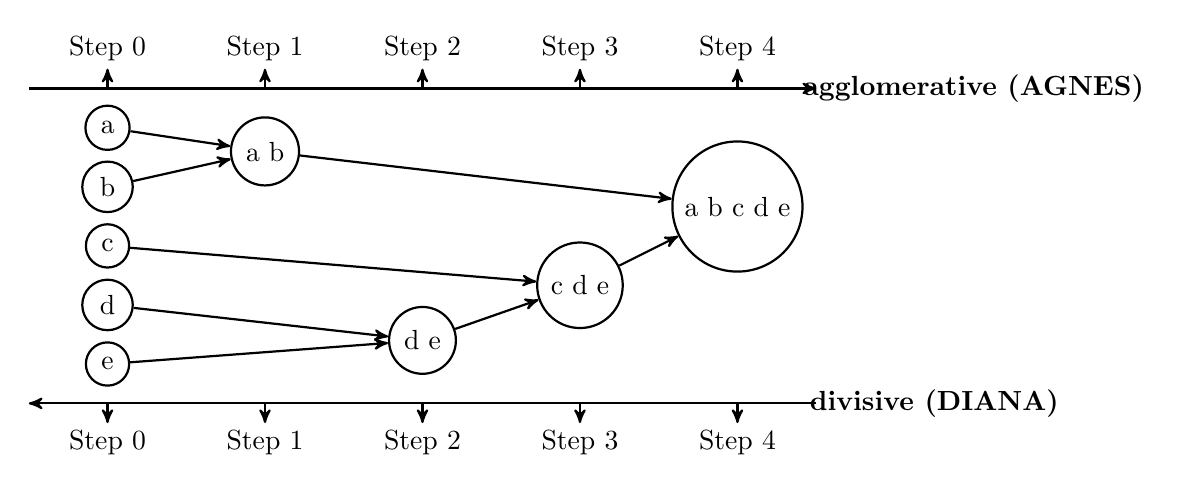
\begin{tikzpicture}[->,>=stealth',auto,node distance=3cm,
  thick,main node/.style={circle,draw}]
          \draw[thick,->] (0,0)--(10,0);
          \draw[thick,->] (10,-4)--(0,-4);
          \draw (1,0)--(1,0.25);
          \node at (1,0.5) {Step 0};
          \draw (3,0)--(3,0.25);
          \node at (3,0.5) {Step 1};
          \draw (5,0)--(5,0.25);
          \node at (5,0.5) {Step 2};
          \draw (7,0)--(7,0.25);
          \node at (7,0.5) {Step 3};
          \draw (9,0)--(9,0.25);
          \node at (9,0.5) {Step 4};
          \draw (1,-4)--(1,-4.25);
          \node at (1,-4.5) {Step 0};
          \draw (3,-4)--(3,-4.25);
          \node at (3,-4.5) {Step 1};
          \draw (5,-4)--(5,-4.25);
          \node at (5,-4.5) {Step 2};
          \draw (7,-4)--(7,-4.25);
          \node at (7,-4.5) {Step 3};
          \draw (9,-4)--(9,-4.25);
          \node at (9,-4.5) {Step 4};
          \node[main node] at (1,-0.5) (a) {a};
          \node[main node] at (1,-1.25) (b) {b};
          \node[main node] at (1,-2) (c) {c};
          \node[main node] at (1,-2.75) (d) {d};
          \node[main node] at (1,-3.5) (e) {e};
          \node[main node] at (3,-0.8) (ab) {a b};
          \node[main node] at (5,-3.2) (de) {d e};
          \node[main node] at (7,-2.5) (cde) {c d e};
          \node[main node] at (9,-1.5) (abcde) {a b c d e};
          \draw (a)--(ab);
          \draw (b)--(ab);
          \draw (ab)--(abcde);
          \draw (c)--(cde);
          \draw (d)--(de);
          \draw (e)--(de);
          \draw (de)--(cde);
          \draw (cde)--(abcde);
          \node at (11.5,-4) {\textbf{divisive (DIANA)}};
          \node at (12,0) {\textbf{agglomerative (AGNES)}};
        \end{tikzpicture}
    \end{frame}
  }

  { % Questions?
    \setbeamertemplate{footline}{}
    \begin{frame}{AGNES (Agglomerative Nesting)}
      \begin{itemize}
        \item \textbf{Introduced in (Kaufmann \& Rousseeuw, 1990)}
        \item \textbf{Implemented in statistical packages, e.g., S+.}
        \item \textbf{Use the single-link method.} (see below)
        \item \textbf{Merge nodes that have the least dissimilarity.}
        \item \textbf{Go on in a non-descending fashion.}
        \item \textbf{Eventually all nodes belong to the same cluster.}
      \end{itemize}
      \newcommand*{\xMin}{0}%
      \newcommand*{\xMax}{10}%
      \newcommand*{\yMin}{0}%
      \newcommand*{\yMax}{10}%
      \centering
      \begin{tikzpicture}[scale=0.23]
          \foreach \i in {\xMin,...,\xMax} {
              \draw [very thin,gray] (\i,\yMin) -- (\i,\yMax)  node [below] at (\i,\yMin) {\tiny$\i$};
          }
          \foreach \i in {\yMin,...,\yMax} {
              \draw [very thin,gray] (\xMin,\i) -- (\xMax,\i) node [left] at (\xMin,\i) {\tiny$\i$};
          }
          \node[color=orange] at (2,6) {\Huge\textbullet};
          \node[color=orange] at (3,4) {\Huge\textbullet};
          \node[color=orange] at (3,8) {\Huge\textbullet};
          \node[color=orange] at (4,5) {\Huge\textbullet};
          \node[color=orange] at (4,7) {\Huge\textbullet};
          \node[color=orange] at (6,2) {\Huge\textbullet};
          \node[color=orange] at (7,2) {\Huge\textbullet};
          \node[color=orange] at (7,4) {\Huge\textbullet};
          \node[color=orange] at (8,4) {\Huge\textbullet};
          \node[color=orange] at (8,5) {\Huge\textbullet};
          \draw[->] (12,5)--(17,5);
          \draw[dashed] (3.4,7.5) ellipse (1.5cm and 1.2cm);
          \draw[dashed] (3.5,4.8) ellipse (1.5cm and 1cm);
          \draw[dashed] (8,5) ellipse (1cm and 1.5cm);
      \end{tikzpicture}
      \begin{tikzpicture}[scale=0.23]
          \foreach \i in {\xMin,...,\xMax} {
              \draw [very thin,gray] (\i,\yMin) -- (\i,\yMax)  node [below] at (\i,\yMin) {\tiny$\i$};
          }
          \foreach \i in {\yMin,...,\yMax} {
              \draw [very thin,gray] (\xMin,\i) -- (\xMax,\i) node [left] at (\xMin,\i) {\tiny$\i$};
          }
          \node[color=orange] at (2,6) {\Huge\textbullet};
          \node[color=orange] at (3,4) {\Huge\textbullet};
          \node[color=orange] at (3,8) {\Huge\textbullet};
          \node[color=orange] at (4,5) {\Huge\textbullet};
          \node[color=orange] at (4,7) {\Huge\textbullet};
          \node[color=orange] at (6,2) {\Huge\textbullet};
          \node[color=orange] at (7,2) {\Huge\textbullet};
          \node[color=orange] at (7,4) {\Huge\textbullet};
          \node[color=orange] at (8,4) {\Huge\textbullet};
          \node[color=orange] at (8,5) {\Huge\textbullet};
          \draw[->] (12,5)--(17,5);
          \draw[dashed] (3,7) ellipse (2cm and 1.5cm);
          \draw[dashed] (3.5,4.8) ellipse (1.5cm and 1cm);
          \draw[dashed] (7.5,5) ellipse (1.5cm and 1.5cm);
          \draw[dashed] (6.25,2.5) ellipse (1.5cm and 1cm);
      \end{tikzpicture}
      \begin{tikzpicture}[scale=0.23]
          \foreach \i in {\xMin,...,\xMax} {
              \draw [very thin,gray] (\i,\yMin) -- (\i,\yMax)  node [below] at (\i,\yMin) {\tiny$\i$};
          }
          \foreach \i in {\yMin,...,\yMax} {
              \draw [very thin,gray] (\xMin,\i) -- (\xMax,\i) node [left] at (\xMin,\i) {\tiny$\i$};
          }
          \node[color=orange] at (2,6) {\Huge\textbullet};
          \node[color=orange] at (3,4) {\Huge\textbullet};
          \node[color=orange] at (3,8) {\Huge\textbullet};
          \node[color=orange] at (4,5) {\Huge\textbullet};
          \node[color=orange] at (4,7) {\Huge\textbullet};
          \node[color=orange] at (6,2) {\Huge\textbullet};
          \node[color=orange] at (7,2) {\Huge\textbullet};
          \node[color=orange] at (7,4) {\Huge\textbullet};
          \node[color=orange] at (8,4) {\Huge\textbullet};
          \node[color=orange] at (8,5) {\Huge\textbullet};
          \draw[dashed] (3,6) ellipse (2cm and 3cm);
          \draw[dashed] (7,4) ellipse (2cm and 3cm);
      \end{tikzpicture}
    \end{frame}
  }

  { % Questions?
    \setbeamertemplate{footline}{}
    \begin{frame}{Dendrogram: shows how clusters are merged}
      \begin{itemize}
        \item Decompose data objects into a several levels of nested partitioning (tree of clusters),\\ called a \textbf{\color{airforceblue}dendrogram}.
        \item A clustering of the data objects is obtained by \textbf{\color{airforceblue}cutting} the dendrogram at the desired level,\\ then each connected component forms a cluster.
      \end{itemize}
      \centering
      \resizebox{7cm}{!}{%
      \begin{tikzpicture}[sloped]
        \node (a) at (-6,0) {a};
        \node (b) at (-3,0) {b};
        \node (c) at (-0.5,0) {c};
        \node (d) at (0.5,0) {d};
        \node (e) at (2,0) {e};
        \node (ab) at (-4.5,3) {};
        \node (cd) at (0,1) {};
        \node (cde) at (1,2) {};
        \node (all) at (-1.5,5) {};

        \draw  (a) |- (ab.center);
        \draw  (b) |- (ab.center);
        \draw  (c) |- (cd.center);
        \draw  (d) |- (cd.center);
        \draw  (e) |- (cde.center);
        \draw  (cd.center) |- (cde.center);
        \draw  (ab.center) |- (all.center);
        \draw  (cde.center) |- (all.center);

        \draw[->,-triangle 60] (-7,0) -- node[above]{distance} (-7,6);
      \end{tikzpicture}}
    \end{frame}
  }

  { % Questions?
    \setbeamertemplate{footline}{}
    \begin{frame}{DIANA (Divisive Analysis)}
      \begin{itemize}
        \item \textbf{Introduced in (Kaufmann \& Rousseeuw, 1990)}
        \item \textbf{Implemented in statistical analysis packages, e.g., S+.}
        \item \textbf{Inverse order of AGNES.}
        \item \textbf{Eventually each node forms a cluster of its own.}
      \end{itemize}
      \newcommand*{\xMin}{0}%
      \newcommand*{\xMax}{10}%
      \newcommand*{\yMin}{0}%
      \newcommand*{\yMax}{10}%
      \vspace{0.5cm}
      \centering
      \begin{tikzpicture}[scale=0.23]
          \foreach \i in {\xMin,...,\xMax} {
              \draw [very thin,gray] (\i,\yMin) -- (\i,\yMax)  node [below] at (\i,\yMin) {\tiny$\i$};
          }
          \foreach \i in {\yMin,...,\yMax} {
              \draw [very thin,gray] (\xMin,\i) -- (\xMax,\i) node [left] at (\xMin,\i) {\tiny$\i$};
          }
          \node[color=orange] at (2,6) {\Huge\textbullet};
          \node[color=orange] at (3,4) {\Huge\textbullet};
          \node[color=orange] at (3,8) {\Huge\textbullet};
          \node[color=orange] at (4,5) {\Huge\textbullet};
          \node[color=orange] at (4,7) {\Huge\textbullet};
          \node[color=orange] at (6,2) {\Huge\textbullet};
          \node[color=orange] at (7,2) {\Huge\textbullet};
          \node[color=orange] at (7,4) {\Huge\textbullet};
          \node[color=orange] at (8,4) {\Huge\textbullet};
          \node[color=orange] at (8,5) {\Huge\textbullet};
          \draw[->] (12,5)--(17,5);
          \draw[dashed] (3,6) ellipse (2cm and 3cm);
          \draw[dashed] (7,4) ellipse (2cm and 3cm);
      \end{tikzpicture}
      \begin{tikzpicture}[scale=0.23]
          \foreach \i in {\xMin,...,\xMax} {
              \draw [very thin,gray] (\i,\yMin) -- (\i,\yMax)  node [below] at (\i,\yMin) {\tiny$\i$};
          }
          \foreach \i in {\yMin,...,\yMax} {
              \draw [very thin,gray] (\xMin,\i) -- (\xMax,\i) node [left] at (\xMin,\i) {\tiny$\i$};
          }
          \node[color=orange] at (2,6) {\Huge\textbullet};
          \node[color=orange] at (3,4) {\Huge\textbullet};
          \node[color=orange] at (3,8) {\Huge\textbullet};
          \node[color=orange] at (4,5) {\Huge\textbullet};
          \node[color=orange] at (4,7) {\Huge\textbullet};
          \node[color=orange] at (6,2) {\Huge\textbullet};
          \node[color=orange] at (7,2) {\Huge\textbullet};
          \node[color=orange] at (7,4) {\Huge\textbullet};
          \node[color=orange] at (8,4) {\Huge\textbullet};
          \node[color=orange] at (8,5) {\Huge\textbullet};
          \draw[->] (12,5)--(17,5);
          \draw[dashed] (3,7) ellipse (2cm and 1.5cm);
          \draw[dashed] (3.5,4.8) ellipse (1.5cm and 1cm);
          \draw[dashed] (7.5,5) ellipse (1.5cm and 1.5cm);
          \draw[dashed] (6.25,2.5) ellipse (1.5cm and 1cm);
      \end{tikzpicture}
      \begin{tikzpicture}[scale=0.23]
          \foreach \i in {\xMin,...,\xMax} {
              \draw [very thin,gray] (\i,\yMin) -- (\i,\yMax)  node [below] at (\i,\yMin) {\tiny$\i$};
          }
          \foreach \i in {\yMin,...,\yMax} {
              \draw [very thin,gray] (\xMin,\i) -- (\xMax,\i) node [left] at (\xMin,\i) {\tiny$\i$};
          }
          \node[color=orange] at (2,6) {\Huge\textbullet};
          \node[color=orange] at (3,4) {\Huge\textbullet};
          \node[color=orange] at (3,8) {\Huge\textbullet};
          \node[color=orange] at (4,5) {\Huge\textbullet};
          \node[color=orange] at (4,7) {\Huge\textbullet};
          \node[color=orange] at (6,2) {\Huge\textbullet};
          \node[color=orange] at (7,2) {\Huge\textbullet};
          \node[color=orange] at (7,4) {\Huge\textbullet};
          \node[color=orange] at (8,4) {\Huge\textbullet};
          \node[color=orange] at (8,5) {\Huge\textbullet};
          \draw[dashed] (3.4,7.5) ellipse (1.5cm and 1.2cm);
          \draw[dashed] (3.5,4.8) ellipse (1.5cm and 1cm);
          \draw[dashed] (8,5) ellipse (1cm and 1.5cm);
          \draw[dashed] (7,4.3) ellipse (0.8cm and 0.8cm);
          \draw[dashed] (6.25,2.5) ellipse (1.5cm and 1cm);
          \draw[dashed] (2,6) ellipse (0.8cm and 0.8cm);
      \end{tikzpicture}
    \end{frame}
  }

  { % Questions?
    \setbeamertemplate{footline}{}
    \begin{frame}{Distance between clusters}
      \begin{itemize}
        \item \textbf{Minimum distance:}
        \begin{itemize}
          \item Smallest distance between an object in one cluster and an object in the other, i.e., $\text{dist}_{\text{min}} (C_i, C_j) = \text{min}_{o_{ip} \in C_i, o_{jq} \in C_j} d(o_{ip}, o_{jq})$.
        \end{itemize}
        \item \textbf{Maximum distance:}
        \begin{itemize}
          \item Largest distance between an object in one cluster and an object in the other, i.e., $\text{dist}_\text{max}(C_i, C_j) = \text{max}_{o_{ip} \in C_i, o_{jq} \in C_j} d(o_{ip}, o_{jq}).$
        \end{itemize}
        \item \textbf{Average distance:}
        \begin{itemize}
          \item Average distance between an object in one cluster and an object in the other, i.e., $\text{dist}_{\text{avg}} (C_i, C_j) = \frac{1}{n_i \cdot n_j} \sum_{o_{ip} \in C_i, o_{jq} \in C_j} d(o_{ip}, o_{jq}).$
        \end{itemize}
        \item \textbf{Mean distance:}
        \begin{itemize}
          \item Distance between the centroids of two clusters, i.e., $\text{dist}_{\text{mean}} (C_i, C_j) = d(c_i, c_j).$
        \end{itemize}
      \end{itemize}
    \end{frame}
  }

  { % Questions?
    \setbeamertemplate{footline}{}
    \begin{frame}{Distance between clusters (II)}
      \begin{itemize}
        \item \textbf{Nearest-neighbor clustering algorithm:}
        \begin{itemize}
          \item Uses \textbf{\color{airforceblue}minimum distance} to measure distance between clusters.
        \end{itemize}
        \item \textbf{Single-linkage algorithm:}
        \begin{itemize}
          \item Terminates if distance between nearest clusters exceeds user-defined threshold.
        \end{itemize}
        \item \textbf{Minimal spanning-tree algorithm:}
        \begin{itemize}
          \item View objects (data points) as nodes of a graph.
          \item Edges form a path between nodes in a cluster.
          \item Merging of two clusters corresponds to adding an edge between the nearest pair of nodes.
          \item Because edges linking clusters always go between distinct clusters,\\
          resulting graph will be a tree.
          \item Thus, agglomerative hierarchical clustering that uses minimum distance produces minimal spanning tree.
        \end{itemize}
      \end{itemize}
    \end{frame}
  }

  { % Questions?
    \setbeamertemplate{footline}{}
    \begin{frame}{Distance between clusters (III)}
      \begin{itemize}
        \item \textbf{Farthest-neighbor clustering algorithm:}
        \begin{itemize}
          \item Uses \textbf{\color{airforceblue}maximum distance} to measure distance between clusters.
        \end{itemize}
        \item \textbf{Complete-linkage algorithm:}
        \begin{itemize}
          \item Terminates if maximum distance between nearest clusters exceeds user-defined threshold.
          \item Good if true clusters are rather compact and approx. equal in size.
        \end{itemize}
      \end{itemize}
    \end{frame}
  }

  { % Questions?
    \setbeamertemplate{footline}{}
    \begin{frame}{Extensions to hierarchical clustering}
      \begin{itemize}
        \item \textbf{Major weakness of agglomerative clustering methods:}
        \begin{itemize}
          \item Can never undo what was done previously.
          \item Do not scale well: Time complexity of at least $\mathcal{O}(n^2)$, where $n$ is the number of objects.
        \end{itemize}
        \item \textbf{Integration of hierarchical and distance-based clustering:}
        \begin{itemize}
          \item BIRCH (1996): Uses CF-tree and incrementally adjusts the quality of sub-clusters.
          \item CHAMELEON (1999): Hierarchical clustering using dynamic modeling.
        \end{itemize}
      \end{itemize}
    \end{frame}
  }

  { % Questions?
    \setbeamertemplate{footline}{}
    \begin{frame}{BIRCH (Balanced Iterative Reducing and Clustering Using Hierarchies)}
      \begin{itemize}
        \item (Zhang, Ramakrishnan \& Livny, SIGMOD'96)
        \item \textbf{Incrementally construct a CF (Clustering Feature) tree:}
        \begin{itemize}
          \item A hierarchical data structure for multiphase clustering.
          \item Phase 1: Scan DB to build an initial in-memory CF-tree.
          \begin{itemize}
            \item A multi-level compression of the data that tries to preserve the inherent clustering structure of the data.
          \end{itemize}
          \item Phase 2: Use an arbitrary clustering algorithm to cluster the leaf nodes of the CF-tree.
        \end{itemize}
        \item \textbf{Scales linearly:}
        \begin{itemize}
          \item Finds a good clustering with a single scan and improves the quality with a few additional scans.
        \end{itemize}
        \item \textbf{Weakness:}
        \begin{itemize}
          \item Handles only numerical data, and sensitive to the order of the data records.
        \end{itemize}
      \end{itemize}
    \end{frame}
  }

  { % Questions?
    \setbeamertemplate{footline}{}
    \begin{frame}{Clustering feature in BIRCH}
      \begin{itemize}
        \item \textbf{Clustering Feature CF = (n, LS, SS)}:
        \begin{itemize}
          \item $3$D vector summarizing statistics about clusters.
          \item $n$: number of data points.
          \item LS: linear sum of $N$ points $\sum_{i=1}^{n} x_i$.
          \item SS: sqaure sum of $N$ points $\sum_{i=1}^{n} x_i^2$.
        \end{itemize}
      \end{itemize}
        \newcommand*{\xMin}{0}%
        \newcommand*{\xMax}{10}%
        \newcommand*{\yMin}{0}%
        \newcommand*{\yMax}{10}%
        \centering
        \begin{tikzpicture}[scale=0.3]
            \foreach \i in {\xMin,...,\xMax} {
                \draw [very thin,gray] (\i,\yMin) -- (\i,\yMax)  node [below] at (\i,\yMin) {\tiny$\i$};
            }
            \foreach \i in {\yMin,...,\yMax} {
                \draw [very thin,gray] (\xMin,\i) -- (\xMax,\i) node [left] at (\xMin,\i) {\tiny$\i$};
            }
            \node[color=orange] at (2,6) {\Huge\textbullet};
            \node[color=orange] at (3,4) {\Huge\textbullet};
            \node[color=orange] at (3,8) {\Huge\textbullet};
            \node[color=orange] at (4,5) {\Huge\textbullet};
            \node[color=orange] at (4,7) {\Huge\textbullet};
            \node[color=orange] at (6,2) {\Huge\textbullet};
            \node[color=orange] at (7,2) {\Huge\textbullet};
            \node[color=orange] at (7,4) {\Huge\textbullet};
            \node[color=orange] at (8,4) {\Huge\textbullet};
            \node[color=orange] at (8,5) {\Huge\textbullet};
            \draw[dashed] (3,6) ellipse (2cm and 3cm);
            \draw[dashed] (7,4) ellipse (2cm and 3cm);
            \node[draw] at (18,9) {CF = $(5,(16,30),(54,190))$};
            \node at (18,7) {(3,4)};
            \node at (18,5.7) {(2,6)};
            \node at (18,4.4) {(4,5)};
            \node at (18,3.1) {(4,7)};
            \node at (18,1.8) {(3,8)};
            \draw[->] (16,10) to [out=30,in=30] (3.3,9.5);
      \end{tikzpicture}
    \end{frame}
  }

  { % Questions?
    \setbeamertemplate{footline}{}
    \begin{frame}{Clustering feature in BIRCH (II)}
      \begin{itemize}
        \item \textbf{Allows to derive many useful statistics of a cluster:}
        \begin{itemize}
          \item E.g. centroid: $c_i = \frac{\sum_{i=1}^{n}o_i}{n} = \frac{LS}{n}$.
        \end{itemize}
        \item \textbf{Additive:}
        \begin{itemize}
          \item For two disjoint clusters $C_1$ and $C_2$ with clustering features $CF_1 = (n_1, LS_1, SS_1)$ and $CF_2 = (n_2, LS_2, SS_2)$, the clustering feature of the cluster that is formed by merging $C_1$ and $C_2$ is simply: $CF_1 + CF_2 = (n_1 + n_2, LS_1 + LS_2, SS_1 + SS_2)$.
        \end{itemize}
      \end{itemize}
    \end{frame}
  }

  { % Questions?
    \setbeamertemplate{footline}{}
    \begin{frame}{CF-Tree in BIRCH}
      \begin{itemize}
        \item \textbf{Height-balanced tree.}
        \item \textbf{Stores the clustering features for a hierarchical clustering.}
        \begin{itemize}
          \item Non-leaf nodes store sums of the CFs of their children.
        \end{itemize}
        \item \textbf{Two parameters:}
        \begin{itemize}
          \item \textbf{\color{airforceblue}Branching factor $B$}: max \# of children.
          \item \textbf{\color{airforceblue}Threshold $T$}: maximum diameter of sub-clusters stored at leaf nodes.
          \begin{itemize}
            \item Diameter $D$: average pairwise distance within a cluster, \\
            reflects the tightness of the cluster around the centroid:
            \begin{align}
              D = \sqrt{\frac{\sum_{i=1}^{n} \sum_{j=1}^{n} (o_i-o_j)^2}{n(n-1)}} = \sqrt{\frac{2nSS - 2LS^2}{n(n-1)}}.
            \end{align}
          \end{itemize}
        \end{itemize}
      \end{itemize}
    \end{frame}
  }

  { % Questions?
    \setbeamertemplate{footline}{}
    \begin{frame}{CF-Tree structure}
      \centering
      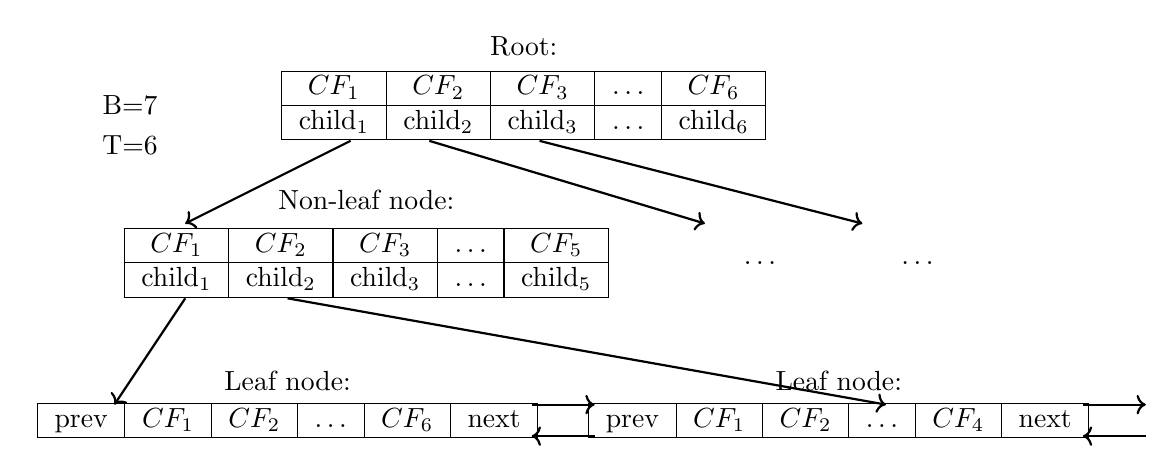
\begin{tikzpicture}
        \node at (0,0.75) {Root:};
        \node at (0,0) {
          \begin{tabular}{|c|c|c|c|c|}
            \hline
            $CF_1$ & $CF_2$ & $CF_3$ & $\hdots$ & $CF_6$ \\ \hline
            $\text{child}_1$ & $\text{child}_2$ & $\text{child}_3$ & $\hdots$ & $\text{child}_6$ \\\hline
          \end{tabular}
        };
        \node at (-2,-1.2) {Non-leaf node:};
        \node at (-2,-2) {
          \begin{tabular}{|c|c|c|c|c|}
            \hline
            $CF_1$ & $CF_2$ & $CF_3$ & $\hdots$ & $CF_5$ \\ \hline
            $\text{child}_1$ & $\text{child}_2$ & $\text{child}_3$ & $\hdots$ & $\text{child}_5$ \\\hline
          \end{tabular}
        };
        \node at (3,-2) {$\hdots$};
        \node at (5,-2) {$\hdots$};
        \node at (-3,-3.5) {Leaf node:};
        \node at (-3,-4) {
          \begin{tabular}{|c|c|c|c|c|c|}
            \hline
            prev & $CF_1$ & $CF_2$ & $\hdots$ & $CF_6$ & next \\ \hline
          \end{tabular}
        };
        \node at (4,-3.5) {Leaf node:};
        \node at (4,-4) {
          \begin{tabular}{|c|c|c|c|c|c|}
            \hline
            prev & $CF_1$ & $CF_2$ & $\hdots$ & $CF_4$ & next \\ \hline
          \end{tabular}
        };
        \draw[thick,->] (-2.2,-0.45)--(-4.3,-1.5);
        \draw[thick,->] (-1.2,-0.45)--(2.3,-1.5);
        \draw[thick,->] (0.2,-0.45)--(4.3,-1.5);
        \draw[thick,->] (-3,-2.45)--(4.6,-3.8);
        \draw[thick,->] (-4.3,-2.45)--(-5.2,-3.8);
        \draw[thick,->] (0.1,-3.8)--(0.9,-3.8);
        \draw[thick,->] (0.9,-4.2)--(0.1,-4.2);
        \draw[thick,->] (7.1,-3.8)--(7.9,-3.8);
        \draw[thick,->] (7.9,-4.2)--(7.1,-4.2);
        \node at (-5,0) {B=7};
        \node at (-5,-0.5) {T=6};
      \end{tikzpicture}
    \end{frame}
  }

  { % Questions?
    \setbeamertemplate{footline}{}
    \begin{frame}[c]
      \begin{center}
        Thank you for your attention.\\
        {\bf Any questions about the seventh chapter?}\\[0.5cm]
        Ask them now, or again, drop me a line: \\
        \faSendO \ \texttt{luciano.melodia@fau.de}.
      \end{center}
    \end{frame}
  }
\end{document}
